\documentclass[12pt]{article}

% Set landscape mode and custom margins for page while including space for the footer
\usepackage[includefoot, margin={0.5cm, 0.5cm}, landscape]{geometry}

\usepackage{graphicx}

% Used to reduce the spacing around section headers and titles.
% Format title headers by adjusting font size
% Set the spacing on all sides of the title to 0
\usepackage[compact]{titlesec}
\titleformat{\section}{\normalfont\bfseries}{\thesection}{1em}{}
\titlespacing*{\section}{0pt}{*0}{0pt}

% Reduce spacing around list items
\usepackage{enumitem}
\setlist{nolistsep}

% Set line spacing
\usepackage{setspace}
\singlespacing

% Create a multicolumn layout
% Set the amount of separation between columns
% Draw a vertical rule between the columns
\usepackage{multicol}
\setlength{\columnsep}{1cm}
\setlength{\columnseprule}{0.1pt}

% Add a frame around the content
\usepackage{mdframed}

% Custom footer (and header if I wanted)
\usepackage{fancyhdr}
\pagestyle{fancy}

% Set custom headers and footers for fancyhdr
\fancyhead{}
\fancyfoot[C]{Android Netrunner Summary Sheet v1.0}
\renewcommand{\headrulewidth}{0pt} 	% Remove horizontal rule from header
\renewcommand{\footrulewidth}{0pt}  % Remove horizontal rule from footer

% Custom frame style for mdframed
% The negative margin is needed to fix a weird spacing that I couldn't figure out
\mdfdefinestyle{customFrame}{%
	everyline=true,%
    outerlinewidth = 0.4pt,%
    innertopmargin = -0.3cm}

% Reduce whitespace in the enumerate list environment
\newenvironment{enumerateCustom}
{\begin{enumerate}
  \setlength{\itemsep}{1pt}
  \setlength{\parskip}{0pt}
  \setlength{\parsep}{0pt}}
{\end{enumerate}}

% Reduce whitespace in the itemize list environment
\newenvironment{itemizeCustom}
{\begin{itemize}
  \setlength{\itemsep}{1pt}
  \setlength{\parskip}{0pt}
  \setlength{\parsep}{0pt}}
{\end{itemize}}

% Prevent paragraph indent
\setlength{\parindent}{0pt}

% Custom commands for common image insertion
% "Credit" Images
\newcommand{\credit}{
\includegraphics[scale=0.40]{images/creditLarge.jpg}\hspace{0.3em}}
\newcommand{\creditWithColon}{
\includegraphics[scale=0.40]{images/creditLarge.jpg}\textbf{:}\hspace{0.3em}}
% "Click" Images
\newcommand{\action}{
\includegraphics[scale=0.40]{images/actionLarge.jpg}\hspace{0.3em}}
\newcommand{\actionWithColon}{
\includegraphics[scale=0.40]{images/actionLarge.jpg}\textbf{:}\hspace{0.3em}}
% "Recurring Credit" Images
\newcommand{\recurringCredit}{\includegraphics[scale=0.40]{images/recurringCreditLarge.jpg}\hspace{0.3em}}
\newcommand{\recurringCreditWithColon}{\includegraphics[scale=0.40]{images/recurringCreditLarge.jpg}\textbf{:}\hspace{0.3em}}
% "Link" Images
\newcommand{\link}{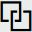
\includegraphics[scale=0.40]{images/linkLarge.jpg}\hspace{0.3em}}
\newcommand{\linkWithColon}{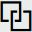
\includegraphics[scale=0.40]{images/linkLarge.jpg}\textbf{:}\hspace{0.3em}}
% "Memory Unit" Images
\newcommand{\memoryUnit}{
\includegraphics[scale=0.40]{images/memoryUnitLarge.jpg}\hspace{0.3em}}
\newcommand{\memoryUnitWithColon}{
\includegraphics[scale=0.40]{images/memoryUnitLarge.jpg}\textbf{:}\hspace{0.3em}}
% "Subroutine" Images
\newcommand{\subroutine}{
\includegraphics[scale=0.40]{images/subroutineLarge.jpg}\hspace{0.3em}}
\newcommand{\subroutineWithColon}{
\includegraphics[scale=0.40]{images/subroutineLarge.jpg}\textbf{:}\hspace{0.3em}}
% "Trash" Images
\newcommand{\trash}{
\includegraphics[scale=0.40]{images/trashLarge.jpg}\hspace{0.3em}}
\newcommand{\trashWithColon}{
\includegraphics[scale=0.40]{images/trashLarge.jpg}\textbf{:}\hspace{0.3em}}

\begin{document}
%\begin{mdframed}[style = customFrame]
\begin{multicols*}{2}

\section*{Setup}
\begin{enumerateCustom}
	\item Pick sides, grab/create decks, and shuffle
	\item Set tokens out in convenient location near both players
	\item 5 \credit to each player
	\item Draw 5 cards for starting hand. Can mulligan \emph{once}.
\end{enumerateCustom}

\section*{Goal of the Game}
\begin{itemizeCustom}
	\item Corporation wins if:
		\begin{itemizeCustom}
			\item Collect 7 \textbf{agenda} points from \textbf{Agenda} cards.
			\item The runner has hand size of less than 0 at end of runner's turn.
			\item The runner takes more damage than the number of cards in his hand.
		\end{itemizeCustom}
	\item Runner wins if:
		\begin{itemizeCustom}
			\item Collect 7 \textbf{agenda} points from \textbf{Agenda} cards.
			\item Corporation has no card in \textbf{R\&D} and attempts to draw.
		\end{itemizeCustom}
\end{itemizeCustom}

\section*{Player Turn}
The Corporation player begins the game. Actions can be performed any number of times in any order.
\begin{enumerateCustom}
	\item \textbf{Draw Phase:} Draw a card from \textbf{R\&D}
	\item \textbf{Action Phase:} Perform 3 actions by spending \action \action \action
	\item \textbf{Discard Phase:} Discard down to maximum hand size, if necessary
\end{enumerateCustom}
Possible actions:
\begin{enumerateCustom}
	\item Draw one card from \textbf{R\&D}
	\item Gain one \credit
	\item Install an \textbf{agenda}, \textbf{asset}, \textbf{upgrade}, or piece of \textbf{ice}
	\item Play an \textbf{operation}
	\item Pay one \creditWithColon Advance a card
	\item Pay two \creditWithColon Trash a Runner's resource if Runner is \textbf{tagged}
	\item Pay \action \action \actionWithColon Purge virus counters.
	\item Trigger \action ability on a card (cost varies).
\end{enumerateCustom}

The Runner player's turn has two phases.
\begin{enumerateCustom}
	\item \textbf{Action Phase:} Perform 4 actions by spending \action \action \action \action
	\item \textbf{Discard Phase:} Discard down to maximum hand size, if necessary
\end{enumerateCustom}
Possible actions:
\begin{enumerateCustom}
	\item Draw one card from the \textbf{stack}
	\item Gain one \credit
	\item Install a \textbf{program}, \textbf{resource}, or piece of \textbf{hardware}
	\item Play an \textbf{event}
	\item Pay two \creditWithColon Remove one \textbf{tag}
	\item Make a run
	\item Trigger \action ability on a card (cost varies).
\end{enumerateCustom}

\section*{Action Explanations}
Corporation: Installing Cards
\begin{itemizeCustom}
	\item \textbf{Assets} and \textbf{upgrades} are played unrezzed. 
	\item When installing, Corp can first \textbf{trash} cards in that server. The trashed cards go to the \textbf{Archives} faceup if rezzed, facedown if unrezzed.
	\item A remote server can be created by installing there. If \textbf{ice} is used, it is \textbf{empty}. Can still be run against.
	\item \textbf{Agendas/Assets:} Can only be installed in remote server. Only one \textbf{agenda} or \textbf{asset} per remote server. \textbf{Upgrades} don't have to be trashed!
	\item \textbf{Upgrades:} Installed in server \textbf{root} when put into central server, otherwise put with agenda/asset. No install limit. Only one \textbf{region} subtype installed per \emph{server}.
	\item \textbf{Ice:} Installed in front of any server (sideways). Installed in outermost position. Must pay cost equal to number of \textbf{ice} in server. Already installed \textbf{ice} may be trashed to reduce install cost.
\end{itemizeCustom}

Corporation: Advancing a Card
\begin{itemizeCustom}
	\item One advancement token placed on installed card. \textbf{Agendas} can always be advanced, others if they state so.
	\item There is no limit to how many times a card can be advanced. 
	\item When \textbf{agenda} is advanced to its advancement requirement, it can be scored. Scoring does \emph{not} cost a \action. Scoring is \emph{not} mandatory.
\end{itemizeCustom}

Runner: Installing Cards
\begin{itemizeCustom}
	\item \textbf{Programs:} Pay install cost, place faceup in program row. If installed programs' memory costs is greater than Runner's memory units, programs must be trashed.
	\item \textbf{Resources:} Pay install cost and place faceup in resource row.
	\item \textbf{Hardware:} Pay install cost and place faceup in hardware row. Limit of one \textbf{console} subtype installed. Can't trash to install another.
\end{itemizeCustom}

Runner: Runs
\\PT - Paid abilities can be triggered. NIR - Non-ice cards can be rezzed.\\
Anything on same line can be resolved in order of choice.
\begin{enumerateCustom}
	\item Declare target server. Get \credit for \textbf{bad publicity}. If ice, goto 2, else goto 4
	\item Runner \textbf{Approaches} outermost unapproached ice.
		\begin{enumerateCustom}
			\item PT
			\item Continue run? If \textbf{Jacks Out} (not first ice of run), goto 6
			\item Approached ice can be rezzed, PT, NIR
			\item If approached ice is rezzed, goto 3. If no more ice, goto 4. If more ice, goto 2.
		\end{enumerateCustom}
	\item Runner \textbf{Encounters} ice (``When encountered'' met)
		\begin{enumerateCustom}
			\item Icebreakers interact with ice, PT
			\item Resolve all unbroken subroutines. If run ends, goto 6. Else, if more ice, goto 2, else goto 4.
		\end{enumerateCustom}
	\item Runner \textbf{Approaches} server
		\begin{enumerateCustom}
			\item PT
			\item Continue run? If \textbf{Jacks Out} goto 6
			\item PT, NIR
			\item Run is successful (``When successful'' met)
			\item Access cards, goto 5. If \textbf{R\&D}, top card + upgrades. If \textbf{HQ}, one random card + upgrades. If \textbf{Archives}, all cards. If \textbf{remote server}, all cards in server but ice.
		\end{enumerateCustom}
	\item Run ends
	\item Run ends and is \textbf{Unsuccessful} (``When unsuccessful'' met)
\end{enumerateCustom}

\section*{Additional Rules}
Traces:
\begin{itemizeCustom}
	\item Some card abilities start a trace. Trace$^{\textrm{x}}$, \textbf{x} is the base strength.
	\item First, Corporation can increase strength by 1 per \credit
	\item Next, Runner can increase link strength by 1 per \credit. Base strength equal to \link in play.
	\item If trace $>$ link, trace is successful. 
\end{itemizeCustom}

Tags
\begin{itemizeCustom}
	\item Some cards place a tag marker on the Runner. When \textbf{tagged}, Corporation can trash resources and Runner can remove tags as an action.
\end{itemizeCustom}

Damage
\begin{itemizeCustom}
	\item \textbf{Meat/Net Damage:} Differ only by name. Runner randomly trashes a card from \textbf{grip} for each such damage.
	\item \textbf{Brain Damage:} Runner randomly trashes one card from \textbf{grip} and reduce hand size by 1.
\end{itemizeCustom}

\end{multicols*}
%\end{mdframed}
\end{document}
